\chapter{The LHC (Large Hadron Collider)}
\label{sec:LHC}

The LHC is the largest circular collider in the world, which is designed to deliver $pp$ collisions with energies up to 14 TeV and instantaneous luminosity up to $10^{34} cm^{-2}s^{-1}$. The instantaneous luminosity is the parameter, representing the proportionality of the event rate and the cross-section for a given process: $N = \mathcal{L} \cdot \sigma$. The parameters is thus process-agnostic, and describes the collider itself in a way that it helps to estimate the amount of collisions happening in the detector. The derivative from this parameter is a pileup, which is the amount of collisions per detector readout. With the increasing of the luminosity, the pileup also increases, flooding the detector with the particles from different processes, making it hard to reconstruct the event. The techniques to overcome the pileup problem will be discussed in Sec.~\ref{sec:Reconstruction}.

The LHC complex includes several accelerators with different sizes of rings which gradually increase the energy of the particles. All of them are shown on the Fig.~\ref{fig:LHC}.

\begin{figure}
\center{
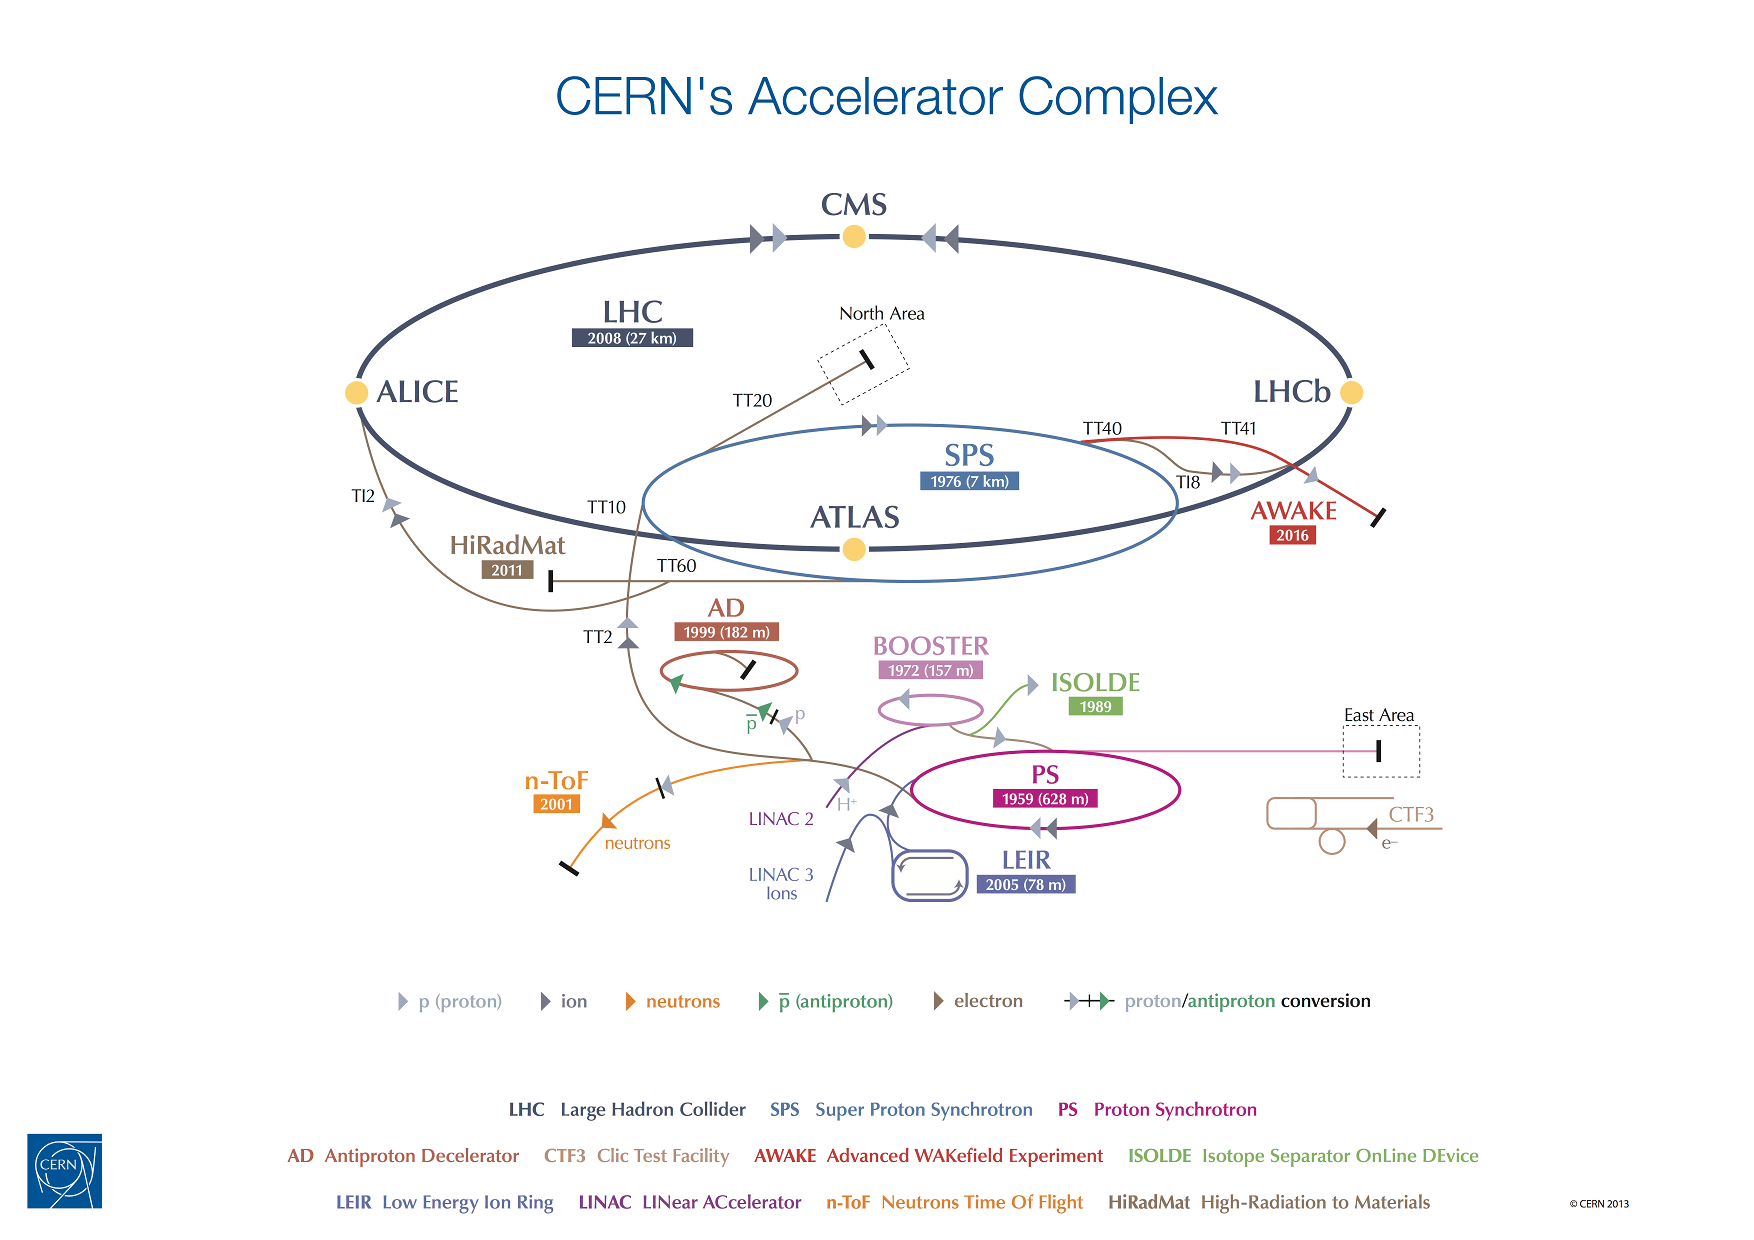
\includegraphics[width=1.0\textwidth]{figures/LHC.jpg}
\caption{The LHC accelerator complex. For each accelerator the year of completion is shown. For circular accelerators the length of the ring is also shown.}
\label{fig:LHC}}
\end{figure}

The full acceleration process of the protons looks like this:

\begin{enumerate}
\item The protons are injected into the Linear Accelerator 2 (Linac2). In case of lead ions Linac3 is used.
\item In case of protons, the bunches are then accelerated in the Proton Synchrotron Booster (Booster), while for heavy ions the Low Energy Ion Ring (LEIR) is used. Both of them pass the accelerated particles to Proton Synchrotron (PS) for storage until the needed amount of particles is pre-accelerated.
\item Next is the Proton Synchrotron - the first high-energy accelerator in this chain, its outputs is 25 GeV, and it was the largest CERN accelerator up until 1970s.
\item The next is the last preparatory accelerator in chain: the Super Proton Synchrotron (SPS). It also once was the most prominent CERN collider and, among other things, lead to the discovery of W and Z bosons during the experiments with \antibar{p} collisions. Its output energy is 450 GeV.
\end{enumerate}

After LHC is filled with the pre-accelerated particles, it starts its own acceleration process. It takes about 20 minutes to reach the energy of 3.5 TeV on which the collision took place during 2011. Next is preparatory stage during which the bunches are focused in order to increase luminosity. If all goes well, the LHC goes into the state of "stable beams": the collisions are started and the detectors can start recording the data. Eventually, the beams loose their focus, the data-taking then stops, and the beams are dumped. The data-taking period is usually several hours long (up to 20) and ideally it lasts as long as the beams circulate the ring, but sometimes other problems arise which prevent data-taking for a period of time during the circulation.

There are 6 detectors which record data from the collisions on LHC.
\begin{itemize}
\item {\bfseries ALICE (A Large Ion Collider Experiment)} This detector is designed to analyze heavy-ion collisions.
\item {\bfseries ATLAS (A Toroidal LHC ApparatuS) and CMS (Compact Muon Solenoid)} These are two general-purpose detectors which cover a wide range of HEP fields. They have differences in design though: ATLAS has less matter in the calorimeter and better muon detectors, while CMS is twice as heavy as ATLAS (has twice as much matter) and because of this has better EM calorimeter, but the detection of hadrons and muons is less precise.
\item {\bfseries LHCb (LHC-beauty)} This detector studies the b-quarks.
\item {\bfseries LHCf (LHC-forward)} This detector studies the forward particles, which behave similar to cosmic rays.
\item {\bfseries TOTEM (TOTal Electric and diffractive cross-section Measurement)} This detector measures the total $pp$ cross-section.
\end{itemize}

Each detector operates independently from one another to enable cross-checking between experiments and increase the trustworthiness of the results.

During 2011 the LHC operated with the same energy of 3.5 TeV per beam and with more or less same luminosity: the difference between the beginning of the data taking in april and the end in december is only about 4 times, as opposed to the ten thousand times, in which the luminosity increased during 2010 data taking. More on the data samples can be seen in Chapter~\ref{sec:DataSamples}.
